\section{Introduction}
\label{sec:intro}

\begin{figure}
  \begin{subfigure}[b]{\columnwidth}
    \centering
    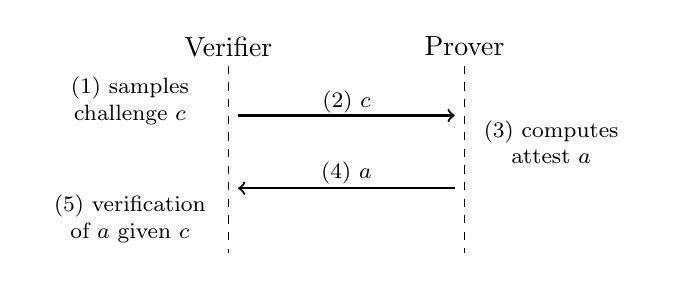
\begin{tikzpicture}[
	squarednode/.style={rectangle, draw=black, thick, minimum size=10mm},
	invisiblenode/.style={rectangle, draw=white}
]
	%Nodes
	\node (verifier) at (0.5,2) {Verifier};
	\node[invisiblenode] (1) at (0.5,1) {};
	\node[invisiblenode] (2) at (0.5,0.2) {};
	\node[invisiblenode] (3) at (0.5,-.75) {};
	
	\node (prover) at (3.5,2) {Prover};
	\node[invisiblenode] (4) at (3.5,1) {};
	\node[invisiblenode] (5) at (3.5,0.2) {};
	\node[invisiblenode] (6) at (3.5,-.75) {};
	
	\node[invisiblenode](sample) at (-0.75,1.3) 
		   {\footnotesize\begin{tabular}{c}(1) samples \\challenge $c$\end{tabular}};
		   \node[invisiblenode](nonce) at (2,1.3) 
		        {\footnotesize(2) $\boldsymbol{c}$};
		        \node[invisiblenode](attest) at (4.6,.75) 
		             {\footnotesize\begin{tabular}{c} (3) computes \\ attest $\boldsymbol{a}$ \end{tabular}};
		             \node[invisiblenode](reply) at (2,0.4) 
		                  {\footnotesize(4) $\boldsymbol{a}$};
		                  \node[invisiblenode](verify) at (-0.75,-0.2)
		                       {\footnotesize\begin{tabular}{c} (5) verification \\ of $\boldsymbol{a}$ given $\boldsymbol{c}$ \end{tabular}};
		                       
		                       %Lines
		                       \draw[dashed]    (verifier.south) -- (3.north);
		                       \draw[dashed]    (prover.south)   -- (6.north);
		                       \draw[->, thick] (1.north east)   -- (4.north west);
		                       \draw[<-, thick] (2.east)         -- (5.west);
		                       
\end{tikzpicture}



    \caption{Protocol}
    \label{fig:problem:prot}
  \end{subfigure}
\\
\\
  \begin{subfigure}[b]{\columnwidth}
    \centering
	  \subsection{Problem Formulation}

% We begin by formulating the problem of dynamic benchmarking for LLMs.
A dynamic benchmark is defined as  
$
\small
\mathcal{B}_{\text{dynamic}} = (\mathcal{D}, T(\cdot)), \quad 
\mathcal{D} = (\mathcal{X}, \mathcal{Y}, \mathcal{S}(\cdot))
$
where \( \mathcal{D} \) represents the static benchmark dataset. 
% consisting of input prompts \( \mathcal{X} \), expected outputs \( \mathcal{Y} \), and a scoring function \( \mathcal{S}(\cdot) \) that evaluates the quality of an LLM's outputs by comparing them against \( \mathcal{Y} \). 
The transformation function \( T(\cdot) \) modifies the data set during the benchmarking to avoid possible data contamination.
The dynamic dataset for the evaluation of an LLM can then be expressed as
$
\small
        \mathcal{D}_t = T_t(\mathcal{D}),  \quad
        \forall t \in \{1, \dots, N\}
$
where \( \mathcal{D}_t \) represents the evaluation data set at the timestamp \( t \), and \( N\) is the total timestamp number, which could be finite or infinite. % \ie $N= \infty$.
If the seed dataset $\mathcal{D}$ is empty, the dynamic benchmarking dataset will be created from scratch.


    \caption{Excerpt \tpm 2.0 spec}
    \label{fig:problem:spec}
  \end{subfigure}

	  \caption{
      %
      The \tpm spec 2.0 specifies remote attestation
      in raw C code.
      %
      We annotated the implict assumptions and
      highlighted our contributions of this paper.
    %
  }
  \label{fig:problem}
\end{figure}


%%
%% What is the problem?
%%

%
Remote attestation (\ra) is a fundamental security protocol for establishing authenticity in many digital systems. 
%
Nevertheless, \ra lacks a rigorous formal specification to
prove \emph{semantic security}--the strongest notion of security.
%
%%
%% Context
%% (More detailed explanation to emphasize that
%%  the problem is actually an important one.)
%%
%

Remote attestation is a protocol verifying that a device runs
the expected software or even hardware.
%
Such devices span the whole spectrum of our digital world.
%
In large and far remote cloud systems, \ra is the foundation for
trusted execution environments that provide confidential
compute capabilities~\cite{10.1145/2872887.2750422,10.1145/3319535.3354220,10.1145/3319535.3354216}.
%
In even the tiniest embedded devices for the Internet of Things (\iot),
\ra attests that the device boots to the expected state and
can be onboard at an \iot platform~\cite{10.1145/2592798.2592824,10.1145/2897937.2898083,10.1145/3654661}.
%
In all these cases, a trusted (and potentially remote) \emph{verifier}
checks the state of an untrusted, potentially compromised \emph{prover} (as shown in Figure~\ref{fig:problem:prot}).
%
This check establishes the authenticity of the prover state based on
cryptographic primitives.
%

%
Despite this widespread use, remote attestation protocols
often lack rigorous formal specifications, leaving critical
vulnerabilities in environments where trust and confidentiality
are essential.
%
For example, the Trusted Platform Module (\tpm) specification
exemplifies a crucial gap~\cite{tpm-spec}.
%
While the \tpm provides key generation and cryptographic
operations, it lacks formal security guarantees.
%
Indeed, the \tpm spec is defined in literal C code.
%
In Figure~\ref{fig:problem:spec}, we excerpt the attestation
call \texttt{SignAttestInfo} from the spec and annotate
its implicit assumptions and implications.
%
Attestation relies on secure signatures and, as such, 
inherits functional correctness and indistinguishability properties. 
%
Indistinguishability is most important because it fundamentally establishes cryptographic security.
%
From the mathematical principles of random sampling over a
distribution, indistinguishability verifies that an attacker
cannot differentiate between the protocol itself and a semantic
model.
%
That is why such a specification defines \emph{semantic security}.
%

%%
%% Why do existing approaches don't cut it?
%% Why is this a hard problem?
%%

%
Existing formal approaches for \ra often focus on functional
correctness but cannot establish semantic security.
%
Many formal \ra specifications rely on the Dolev-Yao model
for security guarantees~\cite{pornin2005digital, tamarin}.
%
These models can verify correctness but assume cryptography
primitives such as functions for encryption and decryption.
%
That is, they assume \emph{semantic security}.
%
Some frameworks, such at VRASED attempts to
fill this gap with informal pen-and-paper proofs~\cite{vrased}.
%
However, without machine-checked evidence, these proofs may harbour
errors or omissions.
%
We are unaware of any formal specification that proves remote
attestation semantically secure.
%

%
This lack may be due to the fact that proving semantic security
is challenging in particular, and appropriate reasoning frameworks
were only established very recently.
%
Frameworks for cryptographic reasoning like CertiCrypt~\cite{barthe2009formal}
and (its extension) EasyCrypt~\cite{barthe2012easycrypt}
have existed for a decade but remained hard to apply.
%
A novel methodology called state-separating proofs (\ssp) allows
reasoning in a modular way about semantic security~\cite{ssp}.
%
However, the integration of \ssp into EasyCrypt~\cite{9919671} and
the introduction of entirely new \ssp{-based} frameworks such as
\ssprove{~\cite{ssprove}}, only happened very recently.
%


%%
%% What is our new insight?
%%

%
Pen-and-paper specifications for the semantic security of \ra
and formally verified digital signature schemes rely
on a different notion of security: (strong) existential unforgeability~\cite{vrased,dupressoir2021machine}.
%
Yet, new frameworks, such as \ssprove establishes semantic
security via indistinguishability.
%
To bridge this gap, we generalize strong existential unforgeability to
indistinguishability.
%

%%
%% What is our approach?
%%

%
Based on this generalization, we formally verify the semantic security
of remote attestation in \ssprove, a framework for modular cryptographic
reasoning in the \coq\footnote{Previously named as Coq}~\cite{coq1996}.
%
We favored \ssprove primarily for two reasons.
%
First, \ssprove provides access to the rich mathematical ecosystem of the \coq, particularly, the mathematical components library~\cite{mahboubi2021mathematical}.
%
Second, \ssprove has a backend in the hax transpiler that allows
us to connect a Rust library implementation for RA with our specification
in a formally verified way~\cite{10.1145/3636501.3636961}.
%
As stated in Figure~\ref{fig:problem}, we establish the implicit assumptions
of the \tpm spec.
%
We verify functional correctness, too, but focus primarily on
indistinguishability.
%

%%
%% Contribution list
%% (What do we provide and
%%  what do we *not* provide (focus of the paper) and
%%  why.)
%%

%
Our paper makes the following contributions:
%
\begin{itemize}
  %
  \item We present the generalization of \emph{strong
  unforgeability} to \emph{perfect indistinguishability} in Section~\ref{sec:TheoryFound} 
  with a brief background knowledge of \ssprove. 
  %
  \item Sections~\ref{sec:sig} and~\ref{sec:vra} define formal 
        specifications of digital signatures and \ra, respectively.
  %After Section~\ref{sec:ssprove} briefly introduced
    %\ssprove, we define our formal specification of \ra.
    %
    Our development reduces the security of remote
    attestations to the security of secure signatures.
    %
    To the best of our knowledge, we provide the first
    machine-checked proof for security against forgery
    of remote attestation (Section~\ref{sec:vra}).
    %
    Our specification of digital signatures is also
    the first in the context of indistinguishability
    proofs.
    %
  \item Our formalization generalizes over specific
    implementations for secure signatures.
    %
    To verify our assumptions on the functional correctness
    of the signatures are sufficient, we instantiate RSA-based
    signatures in Section~\ref{sec:rsa}.
    %
    To the best of our knowledge, our development contains
    the first formally verified key generation for RSA.
    %
  \item During our development, we discovered that the
    assumptions of tools such as \ssprove and the textbook
    definitions for indistinguishability diverge.
    %
    We discuss the implications of our findings for future
    frameworks to reason about indistinguishability in
    Section~\ref{sec:imply} and conclude the paper
    (Section~\ref{sec:concl}). 
\end{itemize}

%%
%% Outlook for the rest of the paper
%% (inlined above)
%%

%
For the final version of the paper, we open-source our
entire \coq development.
%

